% Created by tikzDevice version 0.10.1.2 on 2018-03-05 22:22:06
% !TEX encoding = UTF-8 Unicode
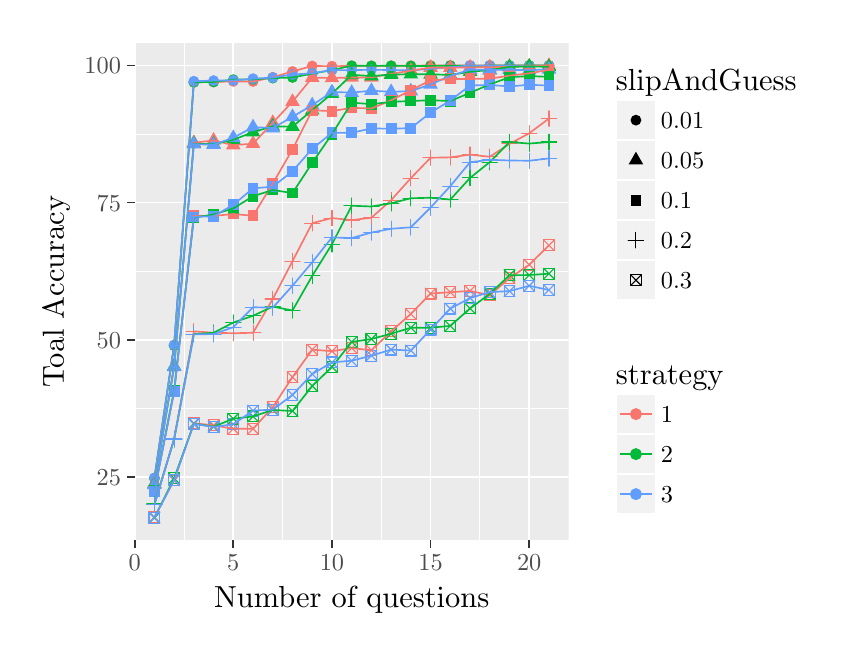
\begin{tikzpicture}[x=1pt,y=1pt]
\definecolor{fillColor}{RGB}{255,255,255}
\path[use as bounding box,fill=fillColor,fill opacity=0.00] (0,0) rectangle (289.08,216.81);
\begin{scope}
\path[clip] (  0.00,  0.00) rectangle (289.08,216.81);
\definecolor{drawColor}{RGB}{255,255,255}
\definecolor{fillColor}{RGB}{255,255,255}

\path[draw=drawColor,line width= 0.6pt,line join=round,line cap=round,fill=fillColor] (  0.00,  0.00) rectangle (289.08,216.81);
\end{scope}
\begin{scope}
\path[clip] ( 38.67, 31.53) rectangle (195.49,211.31);
\definecolor{fillColor}{gray}{0.92}

\path[fill=fillColor] ( 38.67, 31.53) rectangle (195.49,211.31);
\definecolor{drawColor}{RGB}{255,255,255}

\path[draw=drawColor,line width= 0.3pt,line join=round] ( 38.67, 79.28) --
	(195.49, 79.28);

\path[draw=drawColor,line width= 0.3pt,line join=round] ( 38.67,128.82) --
	(195.49,128.82);

\path[draw=drawColor,line width= 0.3pt,line join=round] ( 38.67,178.37) --
	(195.49,178.37);

\path[draw=drawColor,line width= 0.3pt,line join=round] ( 56.49, 31.53) --
	( 56.49,211.31);

\path[draw=drawColor,line width= 0.3pt,line join=round] ( 92.13, 31.53) --
	( 92.13,211.31);

\path[draw=drawColor,line width= 0.3pt,line join=round] (127.77, 31.53) --
	(127.77,211.31);

\path[draw=drawColor,line width= 0.3pt,line join=round] (163.41, 31.53) --
	(163.41,211.31);

\path[draw=drawColor,line width= 0.6pt,line join=round] ( 38.67, 54.51) --
	(195.49, 54.51);

\path[draw=drawColor,line width= 0.6pt,line join=round] ( 38.67,104.05) --
	(195.49,104.05);

\path[draw=drawColor,line width= 0.6pt,line join=round] ( 38.67,153.59) --
	(195.49,153.59);

\path[draw=drawColor,line width= 0.6pt,line join=round] ( 38.67,203.14) --
	(195.49,203.14);

\path[draw=drawColor,line width= 0.6pt,line join=round] ( 38.67, 31.53) --
	( 38.67,211.31);

\path[draw=drawColor,line width= 0.6pt,line join=round] ( 74.31, 31.53) --
	( 74.31,211.31);

\path[draw=drawColor,line width= 0.6pt,line join=round] (109.95, 31.53) --
	(109.95,211.31);

\path[draw=drawColor,line width= 0.6pt,line join=round] (145.59, 31.53) --
	(145.59,211.31);

\path[draw=drawColor,line width= 0.6pt,line join=round] (181.23, 31.53) --
	(181.23,211.31);
\definecolor{fillColor}{RGB}{248,118,109}

\path[fill=fillColor] ( 45.80, 54.08) circle (  1.96);

\path[fill=fillColor] ( 52.92,101.94) circle (  1.96);

\path[fill=fillColor] ( 60.05,197.07) circle (  1.96);

\path[fill=fillColor] ( 67.18,197.17) circle (  1.96);

\path[fill=fillColor] ( 74.31,197.40) circle (  1.96);

\path[fill=fillColor] ( 81.44,197.34) circle (  1.96);

\path[fill=fillColor] ( 88.57,198.90) circle (  1.96);

\path[fill=fillColor] ( 95.69,200.99) circle (  1.96);

\path[fill=fillColor] (102.82,202.98) circle (  1.96);

\path[fill=fillColor] (109.95,202.88) circle (  1.96);

\path[fill=fillColor] (117.08,202.99) circle (  1.96);

\path[fill=fillColor] (124.21,202.99) circle (  1.96);

\path[fill=fillColor] (131.34,203.02) circle (  1.96);

\path[fill=fillColor] (138.46,203.07) circle (  1.96);

\path[fill=fillColor] (145.59,203.14) circle (  1.96);

\path[fill=fillColor] (152.72,203.13) circle (  1.96);

\path[fill=fillColor] (159.85,203.13) circle (  1.96);

\path[fill=fillColor] (166.98,203.13) circle (  1.96);

\path[fill=fillColor] (174.11,203.11) circle (  1.96);

\path[fill=fillColor] (181.23,203.14) circle (  1.96);

\path[fill=fillColor] (188.36,203.14) circle (  1.96);
\definecolor{fillColor}{RGB}{0,186,56}

\path[fill=fillColor] ( 45.80, 53.96) circle (  1.96);

\path[fill=fillColor] ( 52.92,101.93) circle (  1.96);

\path[fill=fillColor] ( 60.05,197.06) circle (  1.96);

\path[fill=fillColor] ( 67.18,197.20) circle (  1.96);

\path[fill=fillColor] ( 74.31,198.04) circle (  1.96);

\path[fill=fillColor] ( 81.44,198.16) circle (  1.96);

\path[fill=fillColor] ( 88.57,198.57) circle (  1.96);

\path[fill=fillColor] ( 95.69,198.81) circle (  1.96);

\path[fill=fillColor] (102.82,200.21) circle (  1.96);

\path[fill=fillColor] (109.95,201.48) circle (  1.96);

\path[fill=fillColor] (117.08,203.05) circle (  1.96);

\path[fill=fillColor] (124.21,203.00) circle (  1.96);

\path[fill=fillColor] (131.34,203.04) circle (  1.96);

\path[fill=fillColor] (138.46,202.97) circle (  1.96);

\path[fill=fillColor] (145.59,202.99) circle (  1.96);

\path[fill=fillColor] (152.72,203.07) circle (  1.96);

\path[fill=fillColor] (159.85,203.03) circle (  1.96);

\path[fill=fillColor] (166.98,203.11) circle (  1.96);

\path[fill=fillColor] (174.11,203.13) circle (  1.96);

\path[fill=fillColor] (181.23,203.14) circle (  1.96);

\path[fill=fillColor] (188.36,203.14) circle (  1.96);
\definecolor{fillColor}{RGB}{97,156,255}

\path[fill=fillColor] ( 45.80, 54.10) circle (  1.96);

\path[fill=fillColor] ( 52.92,102.19) circle (  1.96);

\path[fill=fillColor] ( 60.05,197.46) circle (  1.96);

\path[fill=fillColor] ( 67.18,197.68) circle (  1.96);

\path[fill=fillColor] ( 74.31,197.73) circle (  1.96);

\path[fill=fillColor] ( 81.44,198.38) circle (  1.96);

\path[fill=fillColor] ( 88.57,198.77) circle (  1.96);

\path[fill=fillColor] ( 95.69,199.88) circle (  1.96);

\path[fill=fillColor] (102.82,200.31) circle (  1.96);

\path[fill=fillColor] (109.95,201.50) circle (  1.96);

\path[fill=fillColor] (117.08,201.45) circle (  1.96);

\path[fill=fillColor] (124.21,201.61) circle (  1.96);

\path[fill=fillColor] (131.34,201.49) circle (  1.96);

\path[fill=fillColor] (138.46,201.39) circle (  1.96);

\path[fill=fillColor] (145.59,201.94) circle (  1.96);

\path[fill=fillColor] (152.72,202.51) circle (  1.96);

\path[fill=fillColor] (159.85,203.11) circle (  1.96);

\path[fill=fillColor] (166.98,203.10) circle (  1.96);

\path[fill=fillColor] (174.11,203.08) circle (  1.96);

\path[fill=fillColor] (181.23,203.11) circle (  1.96);

\path[fill=fillColor] (188.36,203.10) circle (  1.96);
\definecolor{fillColor}{RGB}{248,118,109}

\path[fill=fillColor] ( 45.80, 55.21) --
	( 48.44, 50.63) --
	( 43.15, 50.63) --
	cycle;

\path[fill=fillColor] ( 52.92, 97.37) --
	( 55.57, 92.79) --
	( 50.28, 92.79) --
	cycle;

\path[fill=fillColor] ( 60.05,178.27) --
	( 62.69,173.69) --
	( 57.41,173.69) --
	cycle;

\path[fill=fillColor] ( 67.18,179.11) --
	( 69.82,174.53) --
	( 64.54,174.53) --
	cycle;

\path[fill=fillColor] ( 74.31,177.44) --
	( 76.95,172.87) --
	( 71.67,172.87) --
	cycle;

\path[fill=fillColor] ( 81.44,177.92) --
	( 84.08,173.34) --
	( 78.79,173.34) --
	cycle;

\path[fill=fillColor] ( 88.57,185.50) --
	( 91.21,180.92) --
	( 85.92,180.92) --
	cycle;

\path[fill=fillColor] ( 95.69,193.11) --
	( 98.34,188.53) --
	( 93.05,188.53) --
	cycle;

\path[fill=fillColor] (102.82,201.81) --
	(105.46,197.23) --
	(100.18,197.23) --
	cycle;

\path[fill=fillColor] (109.95,201.67) --
	(112.59,197.09) --
	(107.31,197.09) --
	cycle;

\path[fill=fillColor] (117.08,201.86) --
	(119.72,197.28) --
	(114.44,197.28) --
	cycle;

\path[fill=fillColor] (124.21,201.89) --
	(126.85,197.31) --
	(121.56,197.31) --
	cycle;

\path[fill=fillColor] (131.34,203.18) --
	(133.98,198.60) --
	(128.69,198.60) --
	cycle;

\path[fill=fillColor] (138.46,204.31) --
	(141.11,199.73) --
	(135.82,199.73) --
	cycle;

\path[fill=fillColor] (145.59,205.42) --
	(148.23,200.84) --
	(142.95,200.84) --
	cycle;

\path[fill=fillColor] (152.72,205.38) --
	(155.36,200.80) --
	(150.08,200.80) --
	cycle;

\path[fill=fillColor] (159.85,205.51) --
	(162.49,200.93) --
	(157.21,200.93) --
	cycle;

\path[fill=fillColor] (166.98,205.57) --
	(169.62,200.99) --
	(164.33,200.99) --
	cycle;

\path[fill=fillColor] (174.11,205.73) --
	(176.75,201.16) --
	(171.46,201.16) --
	cycle;

\path[fill=fillColor] (181.23,205.92) --
	(183.88,201.35) --
	(178.59,201.35) --
	cycle;

\path[fill=fillColor] (188.36,206.12) --
	(191.00,201.54) --
	(185.72,201.54) --
	cycle;
\definecolor{fillColor}{RGB}{0,186,56}

\path[fill=fillColor] ( 45.80, 54.89) --
	( 48.44, 50.32) --
	( 43.15, 50.32) --
	cycle;

\path[fill=fillColor] ( 52.92, 97.50) --
	( 55.57, 92.92) --
	( 50.28, 92.92) --
	cycle;

\path[fill=fillColor] ( 60.05,177.92) --
	( 62.69,173.34) --
	( 57.41,173.34) --
	cycle;

\path[fill=fillColor] ( 67.18,177.75) --
	( 69.82,173.17) --
	( 64.54,173.17) --
	cycle;

\path[fill=fillColor] ( 74.31,179.35) --
	( 76.95,174.77) --
	( 71.67,174.77) --
	cycle;

\path[fill=fillColor] ( 81.44,182.14) --
	( 84.08,177.56) --
	( 78.79,177.56) --
	cycle;

\path[fill=fillColor] ( 88.57,184.21) --
	( 91.21,179.63) --
	( 85.92,179.63) --
	cycle;

\path[fill=fillColor] ( 95.69,184.06) --
	( 98.34,179.49) --
	( 93.05,179.49) --
	cycle;

\path[fill=fillColor] (102.82,190.06) --
	(105.46,185.48) --
	(100.18,185.48) --
	cycle;

\path[fill=fillColor] (109.95,196.02) --
	(112.59,191.45) --
	(107.31,191.45) --
	cycle;

\path[fill=fillColor] (117.08,202.83) --
	(119.72,198.25) --
	(114.44,198.25) --
	cycle;

\path[fill=fillColor] (124.21,202.37) --
	(126.85,197.80) --
	(121.56,197.80) --
	cycle;

\path[fill=fillColor] (131.34,202.90) --
	(133.98,198.32) --
	(128.69,198.32) --
	cycle;

\path[fill=fillColor] (138.46,203.04) --
	(141.11,198.46) --
	(135.82,198.46) --
	cycle;

\path[fill=fillColor] (145.59,203.02) --
	(148.23,198.44) --
	(142.95,198.44) --
	cycle;

\path[fill=fillColor] (152.72,202.77) --
	(155.36,198.19) --
	(150.08,198.19) --
	cycle;

\path[fill=fillColor] (159.85,203.94) --
	(162.49,199.36) --
	(157.21,199.36) --
	cycle;

\path[fill=fillColor] (166.98,204.53) --
	(169.62,199.96) --
	(164.33,199.96) --
	cycle;

\path[fill=fillColor] (174.11,205.70) --
	(176.75,201.13) --
	(171.46,201.13) --
	cycle;

\path[fill=fillColor] (181.23,205.84) --
	(183.88,201.27) --
	(178.59,201.27) --
	cycle;

\path[fill=fillColor] (188.36,205.71) --
	(191.00,201.14) --
	(185.72,201.14) --
	cycle;
\definecolor{fillColor}{RGB}{97,156,255}

\path[fill=fillColor] ( 45.80, 54.62) --
	( 48.44, 50.05) --
	( 43.15, 50.05) --
	cycle;

\path[fill=fillColor] ( 52.92, 97.27) --
	( 55.57, 92.70) --
	( 50.28, 92.70) --
	cycle;

\path[fill=fillColor] ( 60.05,177.76) --
	( 62.69,173.18) --
	( 57.41,173.18) --
	cycle;

\path[fill=fillColor] ( 67.18,177.56) --
	( 69.82,172.99) --
	( 64.54,172.99) --
	cycle;

\path[fill=fillColor] ( 74.31,180.09) --
	( 76.95,175.51) --
	( 71.67,175.51) --
	cycle;

\path[fill=fillColor] ( 81.44,183.91) --
	( 84.08,179.34) --
	( 78.79,179.34) --
	cycle;

\path[fill=fillColor] ( 88.57,183.59) --
	( 91.21,179.01) --
	( 85.92,179.01) --
	cycle;

\path[fill=fillColor] ( 95.69,187.65) --
	( 98.34,183.07) --
	( 93.05,183.07) --
	cycle;

\path[fill=fillColor] (102.82,191.87) --
	(105.46,187.29) --
	(100.18,187.29) --
	cycle;

\path[fill=fillColor] (109.95,196.62) --
	(112.59,192.04) --
	(107.31,192.04) --
	cycle;

\path[fill=fillColor] (117.08,196.39) --
	(119.72,191.81) --
	(114.44,191.81) --
	cycle;

\path[fill=fillColor] (124.21,197.08) --
	(126.85,192.51) --
	(121.56,192.51) --
	cycle;

\path[fill=fillColor] (131.34,196.67) --
	(133.98,192.09) --
	(128.69,192.09) --
	cycle;

\path[fill=fillColor] (138.46,196.94) --
	(141.11,192.37) --
	(135.82,192.37) --
	cycle;

\path[fill=fillColor] (145.59,199.37) --
	(148.23,194.80) --
	(142.95,194.80) --
	cycle;

\path[fill=fillColor] (152.72,202.40) --
	(155.36,197.83) --
	(150.08,197.83) --
	cycle;

\path[fill=fillColor] (159.85,204.70) --
	(162.49,200.13) --
	(157.21,200.13) --
	cycle;

\path[fill=fillColor] (166.98,204.57) --
	(169.62,200.00) --
	(164.33,200.00) --
	cycle;

\path[fill=fillColor] (174.11,204.64) --
	(176.75,200.07) --
	(171.46,200.07) --
	cycle;

\path[fill=fillColor] (181.23,204.50) --
	(183.88,199.92) --
	(178.59,199.92) --
	cycle;

\path[fill=fillColor] (188.36,204.80) --
	(191.00,200.23) --
	(185.72,200.23) --
	cycle;
\definecolor{fillColor}{RGB}{248,118,109}

\path[fill=fillColor] ( 43.83, 47.26) --
	( 47.76, 47.26) --
	( 47.76, 51.19) --
	( 43.83, 51.19) --
	cycle;

\path[fill=fillColor] ( 50.96, 83.37) --
	( 54.89, 83.37) --
	( 54.89, 87.29) --
	( 50.96, 87.29) --
	cycle;

\path[fill=fillColor] ( 58.09,146.89) --
	( 62.01,146.89) --
	( 62.01,150.81) --
	( 58.09,150.81) --
	cycle;

\path[fill=fillColor] ( 65.22,146.81) --
	( 69.14,146.81) --
	( 69.14,150.73) --
	( 65.22,150.73) --
	cycle;

\path[fill=fillColor] ( 72.35,147.52) --
	( 76.27,147.52) --
	( 76.27,151.44) --
	( 72.35,151.44) --
	cycle;

\path[fill=fillColor] ( 79.47,146.89) --
	( 83.40,146.89) --
	( 83.40,150.81) --
	( 79.47,150.81) --
	cycle;

\path[fill=fillColor] ( 86.60,158.56) --
	( 90.53,158.56) --
	( 90.53,162.48) --
	( 86.60,162.48) --
	cycle;

\path[fill=fillColor] ( 93.73,170.86) --
	( 97.66,170.86) --
	( 97.66,174.78) --
	( 93.73,174.78) --
	cycle;

\path[fill=fillColor] (100.86,184.99) --
	(104.78,184.99) --
	(104.78,188.91) --
	(100.86,188.91) --
	cycle;

\path[fill=fillColor] (107.99,184.69) --
	(111.91,184.69) --
	(111.91,188.61) --
	(107.99,188.61) --
	cycle;

\path[fill=fillColor] (115.12,185.88) --
	(119.04,185.88) --
	(119.04,189.80) --
	(115.12,189.80) --
	cycle;

\path[fill=fillColor] (122.24,185.65) --
	(126.17,185.65) --
	(126.17,189.57) --
	(122.24,189.57) --
	cycle;

\path[fill=fillColor] (129.37,188.61) --
	(133.30,188.61) --
	(133.30,192.54) --
	(129.37,192.54) --
	cycle;

\path[fill=fillColor] (136.50,192.25) --
	(140.43,192.25) --
	(140.43,196.17) --
	(136.50,196.17) --
	cycle;

\path[fill=fillColor] (143.63,195.80) --
	(147.55,195.80) --
	(147.55,199.72) --
	(143.63,199.72) --
	cycle;

\path[fill=fillColor] (150.76,196.33) --
	(154.68,196.33) --
	(154.68,200.25) --
	(150.76,200.25) --
	cycle;

\path[fill=fillColor] (157.89,196.32) --
	(161.81,196.32) --
	(161.81,200.25) --
	(157.89,200.25) --
	cycle;

\path[fill=fillColor] (165.01,196.42) --
	(168.94,196.42) --
	(168.94,200.34) --
	(165.01,200.34) --
	cycle;

\path[fill=fillColor] (172.14,197.51) --
	(176.07,197.51) --
	(176.07,201.43) --
	(172.14,201.43) --
	cycle;

\path[fill=fillColor] (179.27,198.36) --
	(183.20,198.36) --
	(183.20,202.29) --
	(179.27,202.29) --
	cycle;

\path[fill=fillColor] (186.40,199.59) --
	(190.32,199.59) --
	(190.32,203.51) --
	(186.40,203.51) --
	cycle;
\definecolor{fillColor}{RGB}{0,186,56}

\path[fill=fillColor] ( 43.83, 47.68) --
	( 47.76, 47.68) --
	( 47.76, 51.60) --
	( 43.83, 51.60) --
	cycle;

\path[fill=fillColor] ( 50.96, 83.77) --
	( 54.89, 83.77) --
	( 54.89, 87.69) --
	( 50.96, 87.69) --
	cycle;

\path[fill=fillColor] ( 58.09,146.21) --
	( 62.01,146.21) --
	( 62.01,150.14) --
	( 58.09,150.14) --
	cycle;

\path[fill=fillColor] ( 65.22,147.34) --
	( 69.14,147.34) --
	( 69.14,151.27) --
	( 65.22,151.27) --
	cycle;

\path[fill=fillColor] ( 72.35,149.54) --
	( 76.27,149.54) --
	( 76.27,153.47) --
	( 72.35,153.47) --
	cycle;

\path[fill=fillColor] ( 79.47,153.96) --
	( 83.40,153.96) --
	( 83.40,157.88) --
	( 79.47,157.88) --
	cycle;

\path[fill=fillColor] ( 86.60,156.20) --
	( 90.53,156.20) --
	( 90.53,160.12) --
	( 86.60,160.12) --
	cycle;

\path[fill=fillColor] ( 93.73,155.08) --
	( 97.66,155.08) --
	( 97.66,159.00) --
	( 93.73,159.00) --
	cycle;

\path[fill=fillColor] (100.86,166.00) --
	(104.78,166.00) --
	(104.78,169.92) --
	(100.86,169.92) --
	cycle;

\path[fill=fillColor] (107.99,176.36) --
	(111.91,176.36) --
	(111.91,180.29) --
	(107.99,180.29) --
	cycle;

\path[fill=fillColor] (115.12,187.76) --
	(119.04,187.76) --
	(119.04,191.68) --
	(115.12,191.68) --
	cycle;

\path[fill=fillColor] (122.24,187.20) --
	(126.17,187.20) --
	(126.17,191.13) --
	(122.24,191.13) --
	cycle;

\path[fill=fillColor] (129.37,188.03) --
	(133.30,188.03) --
	(133.30,191.95) --
	(129.37,191.95) --
	cycle;

\path[fill=fillColor] (136.50,188.34) --
	(140.43,188.34) --
	(140.43,192.27) --
	(136.50,192.27) --
	cycle;

\path[fill=fillColor] (143.63,188.63) --
	(147.55,188.63) --
	(147.55,192.56) --
	(143.63,192.56) --
	cycle;

\path[fill=fillColor] (150.76,188.32) --
	(154.68,188.32) --
	(154.68,192.25) --
	(150.76,192.25) --
	cycle;

\path[fill=fillColor] (157.89,191.32) --
	(161.81,191.32) --
	(161.81,195.24) --
	(157.89,195.24) --
	cycle;

\path[fill=fillColor] (165.01,194.35) --
	(168.94,194.35) --
	(168.94,198.27) --
	(165.01,198.27) --
	cycle;

\path[fill=fillColor] (172.14,196.93) --
	(176.07,196.93) --
	(176.07,200.85) --
	(172.14,200.85) --
	cycle;

\path[fill=fillColor] (179.27,197.37) --
	(183.20,197.37) --
	(183.20,201.30) --
	(179.27,201.30) --
	cycle;

\path[fill=fillColor] (186.40,197.06) --
	(190.32,197.06) --
	(190.32,200.99) --
	(186.40,200.99) --
	cycle;
\definecolor{fillColor}{RGB}{97,156,255}

\path[fill=fillColor] ( 43.83, 47.32) --
	( 47.76, 47.32) --
	( 47.76, 51.25) --
	( 43.83, 51.25) --
	cycle;

\path[fill=fillColor] ( 50.96, 83.40) --
	( 54.89, 83.40) --
	( 54.89, 87.32) --
	( 50.96, 87.32) --
	cycle;

\path[fill=fillColor] ( 58.09,146.46) --
	( 62.01,146.46) --
	( 62.01,150.38) --
	( 58.09,150.38) --
	cycle;

\path[fill=fillColor] ( 65.22,146.71) --
	( 69.14,146.71) --
	( 69.14,150.63) --
	( 65.22,150.63) --
	cycle;

\path[fill=fillColor] ( 72.35,150.85) --
	( 76.27,150.85) --
	( 76.27,154.77) --
	( 72.35,154.77) --
	cycle;

\path[fill=fillColor] ( 79.47,156.79) --
	( 83.40,156.79) --
	( 83.40,160.72) --
	( 79.47,160.72) --
	cycle;

\path[fill=fillColor] ( 86.60,157.37) --
	( 90.53,157.37) --
	( 90.53,161.29) --
	( 86.60,161.29) --
	cycle;

\path[fill=fillColor] ( 93.73,162.98) --
	( 97.66,162.98) --
	( 97.66,166.90) --
	( 93.73,166.90) --
	cycle;

\path[fill=fillColor] (100.86,171.06) --
	(104.78,171.06) --
	(104.78,174.99) --
	(100.86,174.99) --
	cycle;

\path[fill=fillColor] (107.99,176.82) --
	(111.91,176.82) --
	(111.91,180.74) --
	(107.99,180.74) --
	cycle;

\path[fill=fillColor] (115.12,176.86) --
	(119.04,176.86) --
	(119.04,180.78) --
	(115.12,180.78) --
	cycle;

\path[fill=fillColor] (122.24,178.44) --
	(126.17,178.44) --
	(126.17,182.36) --
	(122.24,182.36) --
	cycle;

\path[fill=fillColor] (129.37,178.33) --
	(133.30,178.33) --
	(133.30,182.25) --
	(129.37,182.25) --
	cycle;

\path[fill=fillColor] (136.50,178.55) --
	(140.43,178.55) --
	(140.43,182.48) --
	(136.50,182.48) --
	cycle;

\path[fill=fillColor] (143.63,184.18) --
	(147.55,184.18) --
	(147.55,188.11) --
	(143.63,188.11) --
	cycle;

\path[fill=fillColor] (150.76,188.51) --
	(154.68,188.51) --
	(154.68,192.44) --
	(150.76,192.44) --
	cycle;

\path[fill=fillColor] (157.89,193.95) --
	(161.81,193.95) --
	(161.81,197.88) --
	(157.89,197.88) --
	cycle;

\path[fill=fillColor] (165.01,194.16) --
	(168.94,194.16) --
	(168.94,198.08) --
	(165.01,198.08) --
	cycle;

\path[fill=fillColor] (172.14,193.60) --
	(176.07,193.60) --
	(176.07,197.52) --
	(172.14,197.52) --
	cycle;

\path[fill=fillColor] (179.27,194.24) --
	(183.20,194.24) --
	(183.20,198.16) --
	(179.27,198.16) --
	cycle;

\path[fill=fillColor] (186.40,193.89) --
	(190.32,193.89) --
	(190.32,197.82) --
	(186.40,197.82) --
	cycle;
\definecolor{drawColor}{RGB}{248,118,109}

\path[draw=drawColor,line width= 0.4pt,line join=round,line cap=round] ( 43.02, 44.62) -- ( 48.57, 44.62);

\path[draw=drawColor,line width= 0.4pt,line join=round,line cap=round] ( 45.80, 41.84) -- ( 45.80, 47.39);

\path[draw=drawColor,line width= 0.4pt,line join=round,line cap=round] ( 50.15, 68.31) -- ( 55.70, 68.31);

\path[draw=drawColor,line width= 0.4pt,line join=round,line cap=round] ( 52.92, 65.53) -- ( 52.92, 71.08);

\path[draw=drawColor,line width= 0.4pt,line join=round,line cap=round] ( 57.28,107.06) -- ( 62.83,107.06);

\path[draw=drawColor,line width= 0.4pt,line join=round,line cap=round] ( 60.05,104.29) -- ( 60.05,109.84);

\path[draw=drawColor,line width= 0.4pt,line join=round,line cap=round] ( 64.41,106.59) -- ( 69.96,106.59);

\path[draw=drawColor,line width= 0.4pt,line join=round,line cap=round] ( 67.18,103.81) -- ( 67.18,109.36);

\path[draw=drawColor,line width= 0.4pt,line join=round,line cap=round] ( 71.53,106.39) -- ( 77.08,106.39);

\path[draw=drawColor,line width= 0.4pt,line join=round,line cap=round] ( 74.31,103.61) -- ( 74.31,109.16);

\path[draw=drawColor,line width= 0.4pt,line join=round,line cap=round] ( 78.66,106.56) -- ( 84.21,106.56);

\path[draw=drawColor,line width= 0.4pt,line join=round,line cap=round] ( 81.44,103.78) -- ( 81.44,109.33);

\path[draw=drawColor,line width= 0.4pt,line join=round,line cap=round] ( 85.79,118.75) -- ( 91.34,118.75);

\path[draw=drawColor,line width= 0.4pt,line join=round,line cap=round] ( 88.57,115.98) -- ( 88.57,121.53);

\path[draw=drawColor,line width= 0.4pt,line join=round,line cap=round] ( 92.92,132.43) -- ( 98.47,132.43);

\path[draw=drawColor,line width= 0.4pt,line join=round,line cap=round] ( 95.69,129.65) -- ( 95.69,135.20);

\path[draw=drawColor,line width= 0.4pt,line join=round,line cap=round] (100.05,146.17) -- (105.60,146.17);

\path[draw=drawColor,line width= 0.4pt,line join=round,line cap=round] (102.82,143.40) -- (102.82,148.95);

\path[draw=drawColor,line width= 0.4pt,line join=round,line cap=round] (107.18,148.01) -- (112.73,148.01);

\path[draw=drawColor,line width= 0.4pt,line join=round,line cap=round] (109.95,145.23) -- (109.95,150.78);

\path[draw=drawColor,line width= 0.4pt,line join=round,line cap=round] (114.30,147.26) -- (119.85,147.26);

\path[draw=drawColor,line width= 0.4pt,line join=round,line cap=round] (117.08,144.49) -- (117.08,150.04);

\path[draw=drawColor,line width= 0.4pt,line join=round,line cap=round] (121.43,148.14) -- (126.98,148.14);

\path[draw=drawColor,line width= 0.4pt,line join=round,line cap=round] (124.21,145.37) -- (124.21,150.92);

\path[draw=drawColor,line width= 0.4pt,line join=round,line cap=round] (128.56,154.49) -- (134.11,154.49);

\path[draw=drawColor,line width= 0.4pt,line join=round,line cap=round] (131.34,151.71) -- (131.34,157.26);

\path[draw=drawColor,line width= 0.4pt,line join=round,line cap=round] (135.69,162.43) -- (141.24,162.43);

\path[draw=drawColor,line width= 0.4pt,line join=round,line cap=round] (138.46,159.66) -- (138.46,165.21);

\path[draw=drawColor,line width= 0.4pt,line join=round,line cap=round] (142.82,169.81) -- (148.37,169.81);

\path[draw=drawColor,line width= 0.4pt,line join=round,line cap=round] (145.59,167.04) -- (145.59,172.59);

\path[draw=drawColor,line width= 0.4pt,line join=round,line cap=round] (149.95,169.94) -- (155.50,169.94);

\path[draw=drawColor,line width= 0.4pt,line join=round,line cap=round] (152.72,167.17) -- (152.72,172.72);

\path[draw=drawColor,line width= 0.4pt,line join=round,line cap=round] (157.07,170.93) -- (162.62,170.93);

\path[draw=drawColor,line width= 0.4pt,line join=round,line cap=round] (159.85,168.16) -- (159.85,173.71);

\path[draw=drawColor,line width= 0.4pt,line join=round,line cap=round] (164.20,170.16) -- (169.75,170.16);

\path[draw=drawColor,line width= 0.4pt,line join=round,line cap=round] (166.98,167.39) -- (166.98,172.94);

\path[draw=drawColor,line width= 0.4pt,line join=round,line cap=round] (171.33,174.82) -- (176.88,174.82);

\path[draw=drawColor,line width= 0.4pt,line join=round,line cap=round] (174.11,172.04) -- (174.11,177.59);

\path[draw=drawColor,line width= 0.4pt,line join=round,line cap=round] (178.46,178.65) -- (184.01,178.65);

\path[draw=drawColor,line width= 0.4pt,line join=round,line cap=round] (181.23,175.88) -- (181.23,181.43);

\path[draw=drawColor,line width= 0.4pt,line join=round,line cap=round] (185.59,183.96) -- (191.14,183.96);

\path[draw=drawColor,line width= 0.4pt,line join=round,line cap=round] (188.36,181.19) -- (188.36,186.74);
\definecolor{drawColor}{RGB}{0,186,56}

\path[draw=drawColor,line width= 0.4pt,line join=round,line cap=round] ( 43.02, 44.67) -- ( 48.57, 44.67);

\path[draw=drawColor,line width= 0.4pt,line join=round,line cap=round] ( 45.80, 41.89) -- ( 45.80, 47.44);

\path[draw=drawColor,line width= 0.4pt,line join=round,line cap=round] ( 50.15, 68.03) -- ( 55.70, 68.03);

\path[draw=drawColor,line width= 0.4pt,line join=round,line cap=round] ( 52.92, 65.26) -- ( 52.92, 70.81);

\path[draw=drawColor,line width= 0.4pt,line join=round,line cap=round] ( 57.28,106.07) -- ( 62.83,106.07);

\path[draw=drawColor,line width= 0.4pt,line join=round,line cap=round] ( 60.05,103.30) -- ( 60.05,108.85);

\path[draw=drawColor,line width= 0.4pt,line join=round,line cap=round] ( 64.41,106.56) -- ( 69.96,106.56);

\path[draw=drawColor,line width= 0.4pt,line join=round,line cap=round] ( 67.18,103.78) -- ( 67.18,109.33);

\path[draw=drawColor,line width= 0.4pt,line join=round,line cap=round] ( 71.53,110.26) -- ( 77.08,110.26);

\path[draw=drawColor,line width= 0.4pt,line join=round,line cap=round] ( 74.31,107.49) -- ( 74.31,113.04);

\path[draw=drawColor,line width= 0.4pt,line join=round,line cap=round] ( 78.66,112.72) -- ( 84.21,112.72);

\path[draw=drawColor,line width= 0.4pt,line join=round,line cap=round] ( 81.44,109.95) -- ( 81.44,115.50);

\path[draw=drawColor,line width= 0.4pt,line join=round,line cap=round] ( 85.79,116.01) -- ( 91.34,116.01);

\path[draw=drawColor,line width= 0.4pt,line join=round,line cap=round] ( 88.57,113.24) -- ( 88.57,118.79);

\path[draw=drawColor,line width= 0.4pt,line join=round,line cap=round] ( 92.92,114.62) -- ( 98.47,114.62);

\path[draw=drawColor,line width= 0.4pt,line join=round,line cap=round] ( 95.69,111.85) -- ( 95.69,117.40);

\path[draw=drawColor,line width= 0.4pt,line join=round,line cap=round] (100.05,127.12) -- (105.60,127.12);

\path[draw=drawColor,line width= 0.4pt,line join=round,line cap=round] (102.82,124.34) -- (102.82,129.89);

\path[draw=drawColor,line width= 0.4pt,line join=round,line cap=round] (107.18,138.56) -- (112.73,138.56);

\path[draw=drawColor,line width= 0.4pt,line join=round,line cap=round] (109.95,135.79) -- (109.95,141.34);

\path[draw=drawColor,line width= 0.4pt,line join=round,line cap=round] (114.30,152.47) -- (119.85,152.47);

\path[draw=drawColor,line width= 0.4pt,line join=round,line cap=round] (117.08,149.70) -- (117.08,155.25);

\path[draw=drawColor,line width= 0.4pt,line join=round,line cap=round] (121.43,152.19) -- (126.98,152.19);

\path[draw=drawColor,line width= 0.4pt,line join=round,line cap=round] (124.21,149.41) -- (124.21,154.96);

\path[draw=drawColor,line width= 0.4pt,line join=round,line cap=round] (128.56,153.35) -- (134.11,153.35);

\path[draw=drawColor,line width= 0.4pt,line join=round,line cap=round] (131.34,150.57) -- (131.34,156.12);

\path[draw=drawColor,line width= 0.4pt,line join=round,line cap=round] (135.69,155.17) -- (141.24,155.17);

\path[draw=drawColor,line width= 0.4pt,line join=round,line cap=round] (138.46,152.39) -- (138.46,157.94);

\path[draw=drawColor,line width= 0.4pt,line join=round,line cap=round] (142.82,155.35) -- (148.37,155.35);

\path[draw=drawColor,line width= 0.4pt,line join=round,line cap=round] (145.59,152.57) -- (145.59,158.12);

\path[draw=drawColor,line width= 0.4pt,line join=round,line cap=round] (149.95,154.70) -- (155.50,154.70);

\path[draw=drawColor,line width= 0.4pt,line join=round,line cap=round] (152.72,151.93) -- (152.72,157.48);

\path[draw=drawColor,line width= 0.4pt,line join=round,line cap=round] (157.07,162.51) -- (162.62,162.51);

\path[draw=drawColor,line width= 0.4pt,line join=round,line cap=round] (159.85,159.74) -- (159.85,165.29);

\path[draw=drawColor,line width= 0.4pt,line join=round,line cap=round] (164.20,168.24) -- (169.75,168.24);

\path[draw=drawColor,line width= 0.4pt,line join=round,line cap=round] (166.98,165.46) -- (166.98,171.01);

\path[draw=drawColor,line width= 0.4pt,line join=round,line cap=round] (171.33,175.48) -- (176.88,175.48);

\path[draw=drawColor,line width= 0.4pt,line join=round,line cap=round] (174.11,172.71) -- (174.11,178.26);

\path[draw=drawColor,line width= 0.4pt,line join=round,line cap=round] (178.46,174.93) -- (184.01,174.93);

\path[draw=drawColor,line width= 0.4pt,line join=round,line cap=round] (181.23,172.15) -- (181.23,177.70);

\path[draw=drawColor,line width= 0.4pt,line join=round,line cap=round] (185.59,175.48) -- (191.14,175.48);

\path[draw=drawColor,line width= 0.4pt,line join=round,line cap=round] (188.36,172.71) -- (188.36,178.26);
\definecolor{drawColor}{RGB}{97,156,255}

\path[draw=drawColor,line width= 0.4pt,line join=round,line cap=round] ( 43.02, 44.39) -- ( 48.57, 44.39);

\path[draw=drawColor,line width= 0.4pt,line join=round,line cap=round] ( 45.80, 41.61) -- ( 45.80, 47.16);

\path[draw=drawColor,line width= 0.4pt,line join=round,line cap=round] ( 50.15, 68.16) -- ( 55.70, 68.16);

\path[draw=drawColor,line width= 0.4pt,line join=round,line cap=round] ( 52.92, 65.39) -- ( 52.92, 70.94);

\path[draw=drawColor,line width= 0.4pt,line join=round,line cap=round] ( 57.28,105.98) -- ( 62.83,105.98);

\path[draw=drawColor,line width= 0.4pt,line join=round,line cap=round] ( 60.05,103.21) -- ( 60.05,108.76);

\path[draw=drawColor,line width= 0.4pt,line join=round,line cap=round] ( 64.41,106.09) -- ( 69.96,106.09);

\path[draw=drawColor,line width= 0.4pt,line join=round,line cap=round] ( 67.18,103.32) -- ( 67.18,108.87);

\path[draw=drawColor,line width= 0.4pt,line join=round,line cap=round] ( 71.53,108.58) -- ( 77.08,108.58);

\path[draw=drawColor,line width= 0.4pt,line join=round,line cap=round] ( 74.31,105.80) -- ( 74.31,111.35);

\path[draw=drawColor,line width= 0.4pt,line join=round,line cap=round] ( 78.66,115.79) -- ( 84.21,115.79);

\path[draw=drawColor,line width= 0.4pt,line join=round,line cap=round] ( 81.44,113.02) -- ( 81.44,118.57);

\path[draw=drawColor,line width= 0.4pt,line join=round,line cap=round] ( 85.79,115.63) -- ( 91.34,115.63);

\path[draw=drawColor,line width= 0.4pt,line join=round,line cap=round] ( 88.57,112.86) -- ( 88.57,118.41);

\path[draw=drawColor,line width= 0.4pt,line join=round,line cap=round] ( 92.92,123.56) -- ( 98.47,123.56);

\path[draw=drawColor,line width= 0.4pt,line join=round,line cap=round] ( 95.69,120.79) -- ( 95.69,126.34);

\path[draw=drawColor,line width= 0.4pt,line join=round,line cap=round] (100.05,132.05) -- (105.60,132.05);

\path[draw=drawColor,line width= 0.4pt,line join=round,line cap=round] (102.82,129.28) -- (102.82,134.83);

\path[draw=drawColor,line width= 0.4pt,line join=round,line cap=round] (107.18,141.01) -- (112.73,141.01);

\path[draw=drawColor,line width= 0.4pt,line join=round,line cap=round] (109.95,138.24) -- (109.95,143.78);

\path[draw=drawColor,line width= 0.4pt,line join=round,line cap=round] (114.30,140.79) -- (119.85,140.79);

\path[draw=drawColor,line width= 0.4pt,line join=round,line cap=round] (117.08,138.02) -- (117.08,143.57);

\path[draw=drawColor,line width= 0.4pt,line join=round,line cap=round] (121.43,142.78) -- (126.98,142.78);

\path[draw=drawColor,line width= 0.4pt,line join=round,line cap=round] (124.21,140.01) -- (124.21,145.56);

\path[draw=drawColor,line width= 0.4pt,line join=round,line cap=round] (128.56,144.14) -- (134.11,144.14);

\path[draw=drawColor,line width= 0.4pt,line join=round,line cap=round] (131.34,141.37) -- (131.34,146.92);

\path[draw=drawColor,line width= 0.4pt,line join=round,line cap=round] (135.69,144.67) -- (141.24,144.67);

\path[draw=drawColor,line width= 0.4pt,line join=round,line cap=round] (138.46,141.89) -- (138.46,147.44);

\path[draw=drawColor,line width= 0.4pt,line join=round,line cap=round] (142.82,151.80) -- (148.37,151.80);

\path[draw=drawColor,line width= 0.4pt,line join=round,line cap=round] (145.59,149.03) -- (145.59,154.58);

\path[draw=drawColor,line width= 0.4pt,line join=round,line cap=round] (149.95,159.56) -- (155.50,159.56);

\path[draw=drawColor,line width= 0.4pt,line join=round,line cap=round] (152.72,156.78) -- (152.72,162.33);

\path[draw=drawColor,line width= 0.4pt,line join=round,line cap=round] (157.07,168.20) -- (162.62,168.20);

\path[draw=drawColor,line width= 0.4pt,line join=round,line cap=round] (159.85,165.42) -- (159.85,170.97);

\path[draw=drawColor,line width= 0.4pt,line join=round,line cap=round] (164.20,169.04) -- (169.75,169.04);

\path[draw=drawColor,line width= 0.4pt,line join=round,line cap=round] (166.98,166.27) -- (166.98,171.82);

\path[draw=drawColor,line width= 0.4pt,line join=round,line cap=round] (171.33,168.82) -- (176.88,168.82);

\path[draw=drawColor,line width= 0.4pt,line join=round,line cap=round] (174.11,166.05) -- (174.11,171.60);

\path[draw=drawColor,line width= 0.4pt,line join=round,line cap=round] (178.46,168.72) -- (184.01,168.72);

\path[draw=drawColor,line width= 0.4pt,line join=round,line cap=round] (181.23,165.94) -- (181.23,171.49);

\path[draw=drawColor,line width= 0.4pt,line join=round,line cap=round] (185.59,169.56) -- (191.14,169.56);

\path[draw=drawColor,line width= 0.4pt,line join=round,line cap=round] (188.36,166.78) -- (188.36,172.33);
\definecolor{drawColor}{RGB}{248,118,109}

\path[draw=drawColor,line width= 0.4pt,line join=round,line cap=round] ( 43.83, 38.01) rectangle ( 47.76, 41.93);

\path[draw=drawColor,line width= 0.4pt,line join=round,line cap=round] ( 43.83, 38.01) -- ( 47.76, 41.93);

\path[draw=drawColor,line width= 0.4pt,line join=round,line cap=round] ( 43.83, 41.93) -- ( 47.76, 38.01);

\path[draw=drawColor,line width= 0.4pt,line join=round,line cap=round] ( 50.96, 51.25) rectangle ( 54.89, 55.17);

\path[draw=drawColor,line width= 0.4pt,line join=round,line cap=round] ( 50.96, 51.25) -- ( 54.89, 55.17);

\path[draw=drawColor,line width= 0.4pt,line join=round,line cap=round] ( 50.96, 55.17) -- ( 54.89, 51.25);

\path[draw=drawColor,line width= 0.4pt,line join=round,line cap=round] ( 58.09, 71.92) rectangle ( 62.01, 75.84);

\path[draw=drawColor,line width= 0.4pt,line join=round,line cap=round] ( 58.09, 71.92) -- ( 62.01, 75.84);

\path[draw=drawColor,line width= 0.4pt,line join=round,line cap=round] ( 58.09, 75.84) -- ( 62.01, 71.92);

\path[draw=drawColor,line width= 0.4pt,line join=round,line cap=round] ( 65.22, 71.18) rectangle ( 69.14, 75.11);

\path[draw=drawColor,line width= 0.4pt,line join=round,line cap=round] ( 65.22, 71.18) -- ( 69.14, 75.11);

\path[draw=drawColor,line width= 0.4pt,line join=round,line cap=round] ( 65.22, 75.11) -- ( 69.14, 71.18);

\path[draw=drawColor,line width= 0.4pt,line join=round,line cap=round] ( 72.35, 69.89) rectangle ( 76.27, 73.82);

\path[draw=drawColor,line width= 0.4pt,line join=round,line cap=round] ( 72.35, 69.89) -- ( 76.27, 73.82);

\path[draw=drawColor,line width= 0.4pt,line join=round,line cap=round] ( 72.35, 73.82) -- ( 76.27, 69.89);

\path[draw=drawColor,line width= 0.4pt,line join=round,line cap=round] ( 79.47, 69.91) rectangle ( 83.40, 73.84);

\path[draw=drawColor,line width= 0.4pt,line join=round,line cap=round] ( 79.47, 69.91) -- ( 83.40, 73.84);

\path[draw=drawColor,line width= 0.4pt,line join=round,line cap=round] ( 79.47, 73.84) -- ( 83.40, 69.91);

\path[draw=drawColor,line width= 0.4pt,line join=round,line cap=round] ( 86.60, 77.74) rectangle ( 90.53, 81.67);

\path[draw=drawColor,line width= 0.4pt,line join=round,line cap=round] ( 86.60, 77.74) -- ( 90.53, 81.67);

\path[draw=drawColor,line width= 0.4pt,line join=round,line cap=round] ( 86.60, 81.67) -- ( 90.53, 77.74);

\path[draw=drawColor,line width= 0.4pt,line join=round,line cap=round] ( 93.73, 88.57) rectangle ( 97.66, 92.50);

\path[draw=drawColor,line width= 0.4pt,line join=round,line cap=round] ( 93.73, 88.57) -- ( 97.66, 92.50);

\path[draw=drawColor,line width= 0.4pt,line join=round,line cap=round] ( 93.73, 92.50) -- ( 97.66, 88.57);

\path[draw=drawColor,line width= 0.4pt,line join=round,line cap=round] (100.86, 98.49) rectangle (104.78,102.42);

\path[draw=drawColor,line width= 0.4pt,line join=round,line cap=round] (100.86, 98.49) -- (104.78,102.42);

\path[draw=drawColor,line width= 0.4pt,line join=round,line cap=round] (100.86,102.42) -- (104.78, 98.49);

\path[draw=drawColor,line width= 0.4pt,line join=round,line cap=round] (107.99, 97.95) rectangle (111.91,101.87);

\path[draw=drawColor,line width= 0.4pt,line join=round,line cap=round] (107.99, 97.95) -- (111.91,101.87);

\path[draw=drawColor,line width= 0.4pt,line join=round,line cap=round] (107.99,101.87) -- (111.91, 97.95);

\path[draw=drawColor,line width= 0.4pt,line join=round,line cap=round] (115.12, 99.06) rectangle (119.04,102.98);

\path[draw=drawColor,line width= 0.4pt,line join=round,line cap=round] (115.12, 99.06) -- (119.04,102.98);

\path[draw=drawColor,line width= 0.4pt,line join=round,line cap=round] (115.12,102.98) -- (119.04, 99.06);

\path[draw=drawColor,line width= 0.4pt,line join=round,line cap=round] (122.24, 98.26) rectangle (126.17,102.19);

\path[draw=drawColor,line width= 0.4pt,line join=round,line cap=round] (122.24, 98.26) -- (126.17,102.19);

\path[draw=drawColor,line width= 0.4pt,line join=round,line cap=round] (122.24,102.19) -- (126.17, 98.26);

\path[draw=drawColor,line width= 0.4pt,line join=round,line cap=round] (129.37,105.12) rectangle (133.30,109.04);

\path[draw=drawColor,line width= 0.4pt,line join=round,line cap=round] (129.37,105.12) -- (133.30,109.04);

\path[draw=drawColor,line width= 0.4pt,line join=round,line cap=round] (129.37,109.04) -- (133.30,105.12);

\path[draw=drawColor,line width= 0.4pt,line join=round,line cap=round] (136.50,111.41) rectangle (140.43,115.34);

\path[draw=drawColor,line width= 0.4pt,line join=round,line cap=round] (136.50,111.41) -- (140.43,115.34);

\path[draw=drawColor,line width= 0.4pt,line join=round,line cap=round] (136.50,115.34) -- (140.43,111.41);

\path[draw=drawColor,line width= 0.4pt,line join=round,line cap=round] (143.63,118.76) rectangle (147.55,122.69);

\path[draw=drawColor,line width= 0.4pt,line join=round,line cap=round] (143.63,118.76) -- (147.55,122.69);

\path[draw=drawColor,line width= 0.4pt,line join=round,line cap=round] (143.63,122.69) -- (147.55,118.76);

\path[draw=drawColor,line width= 0.4pt,line join=round,line cap=round] (150.76,119.24) rectangle (154.68,123.16);

\path[draw=drawColor,line width= 0.4pt,line join=round,line cap=round] (150.76,119.24) -- (154.68,123.16);

\path[draw=drawColor,line width= 0.4pt,line join=round,line cap=round] (150.76,123.16) -- (154.68,119.24);

\path[draw=drawColor,line width= 0.4pt,line join=round,line cap=round] (157.89,119.74) rectangle (161.81,123.66);

\path[draw=drawColor,line width= 0.4pt,line join=round,line cap=round] (157.89,119.74) -- (161.81,123.66);

\path[draw=drawColor,line width= 0.4pt,line join=round,line cap=round] (157.89,123.66) -- (161.81,119.74);

\path[draw=drawColor,line width= 0.4pt,line join=round,line cap=round] (165.01,118.18) rectangle (168.94,122.10);

\path[draw=drawColor,line width= 0.4pt,line join=round,line cap=round] (165.01,118.18) -- (168.94,122.10);

\path[draw=drawColor,line width= 0.4pt,line join=round,line cap=round] (165.01,122.10) -- (168.94,118.18);

\path[draw=drawColor,line width= 0.4pt,line join=round,line cap=round] (172.14,124.33) rectangle (176.07,128.26);

\path[draw=drawColor,line width= 0.4pt,line join=round,line cap=round] (172.14,124.33) -- (176.07,128.26);

\path[draw=drawColor,line width= 0.4pt,line join=round,line cap=round] (172.14,128.26) -- (176.07,124.33);

\path[draw=drawColor,line width= 0.4pt,line join=round,line cap=round] (179.27,129.20) rectangle (183.20,133.12);

\path[draw=drawColor,line width= 0.4pt,line join=round,line cap=round] (179.27,129.20) -- (183.20,133.12);

\path[draw=drawColor,line width= 0.4pt,line join=round,line cap=round] (179.27,133.12) -- (183.20,129.20);

\path[draw=drawColor,line width= 0.4pt,line join=round,line cap=round] (186.40,136.19) rectangle (190.32,140.12);

\path[draw=drawColor,line width= 0.4pt,line join=round,line cap=round] (186.40,136.19) -- (190.32,140.12);

\path[draw=drawColor,line width= 0.4pt,line join=round,line cap=round] (186.40,140.12) -- (190.32,136.19);
\definecolor{drawColor}{RGB}{0,186,56}

\path[draw=drawColor,line width= 0.4pt,line join=round,line cap=round] ( 43.83, 37.74) rectangle ( 47.76, 41.66);

\path[draw=drawColor,line width= 0.4pt,line join=round,line cap=round] ( 43.83, 37.74) -- ( 47.76, 41.66);

\path[draw=drawColor,line width= 0.4pt,line join=round,line cap=round] ( 43.83, 41.66) -- ( 47.76, 37.74);

\path[draw=drawColor,line width= 0.4pt,line join=round,line cap=round] ( 50.96, 52.01) rectangle ( 54.89, 55.93);

\path[draw=drawColor,line width= 0.4pt,line join=round,line cap=round] ( 50.96, 52.01) -- ( 54.89, 55.93);

\path[draw=drawColor,line width= 0.4pt,line join=round,line cap=round] ( 50.96, 55.93) -- ( 54.89, 52.01);

\path[draw=drawColor,line width= 0.4pt,line join=round,line cap=round] ( 58.09, 71.76) rectangle ( 62.01, 75.68);

\path[draw=drawColor,line width= 0.4pt,line join=round,line cap=round] ( 58.09, 71.76) -- ( 62.01, 75.68);

\path[draw=drawColor,line width= 0.4pt,line join=round,line cap=round] ( 58.09, 75.68) -- ( 62.01, 71.76);

\path[draw=drawColor,line width= 0.4pt,line join=round,line cap=round] ( 65.22, 70.66) rectangle ( 69.14, 74.58);

\path[draw=drawColor,line width= 0.4pt,line join=round,line cap=round] ( 65.22, 70.66) -- ( 69.14, 74.58);

\path[draw=drawColor,line width= 0.4pt,line join=round,line cap=round] ( 65.22, 74.58) -- ( 69.14, 70.66);

\path[draw=drawColor,line width= 0.4pt,line join=round,line cap=round] ( 72.35, 73.56) rectangle ( 76.27, 77.48);

\path[draw=drawColor,line width= 0.4pt,line join=round,line cap=round] ( 72.35, 73.56) -- ( 76.27, 77.48);

\path[draw=drawColor,line width= 0.4pt,line join=round,line cap=round] ( 72.35, 77.48) -- ( 76.27, 73.56);

\path[draw=drawColor,line width= 0.4pt,line join=round,line cap=round] ( 79.47, 74.36) rectangle ( 83.40, 78.29);

\path[draw=drawColor,line width= 0.4pt,line join=round,line cap=round] ( 79.47, 74.36) -- ( 83.40, 78.29);

\path[draw=drawColor,line width= 0.4pt,line join=round,line cap=round] ( 79.47, 78.29) -- ( 83.40, 74.36);

\path[draw=drawColor,line width= 0.4pt,line join=round,line cap=round] ( 86.60, 76.72) rectangle ( 90.53, 80.65);

\path[draw=drawColor,line width= 0.4pt,line join=round,line cap=round] ( 86.60, 76.72) -- ( 90.53, 80.65);

\path[draw=drawColor,line width= 0.4pt,line join=round,line cap=round] ( 86.60, 80.65) -- ( 90.53, 76.72);

\path[draw=drawColor,line width= 0.4pt,line join=round,line cap=round] ( 93.73, 76.32) rectangle ( 97.66, 80.24);

\path[draw=drawColor,line width= 0.4pt,line join=round,line cap=round] ( 93.73, 76.32) -- ( 97.66, 80.24);

\path[draw=drawColor,line width= 0.4pt,line join=round,line cap=round] ( 93.73, 80.24) -- ( 97.66, 76.32);

\path[draw=drawColor,line width= 0.4pt,line join=round,line cap=round] (100.86, 85.37) rectangle (104.78, 89.30);

\path[draw=drawColor,line width= 0.4pt,line join=round,line cap=round] (100.86, 85.37) -- (104.78, 89.30);

\path[draw=drawColor,line width= 0.4pt,line join=round,line cap=round] (100.86, 89.30) -- (104.78, 85.37);

\path[draw=drawColor,line width= 0.4pt,line join=round,line cap=round] (107.99, 92.25) rectangle (111.91, 96.17);

\path[draw=drawColor,line width= 0.4pt,line join=round,line cap=round] (107.99, 92.25) -- (111.91, 96.17);

\path[draw=drawColor,line width= 0.4pt,line join=round,line cap=round] (107.99, 96.17) -- (111.91, 92.25);

\path[draw=drawColor,line width= 0.4pt,line join=round,line cap=round] (115.12,101.31) rectangle (119.04,105.23);

\path[draw=drawColor,line width= 0.4pt,line join=round,line cap=round] (115.12,101.31) -- (119.04,105.23);

\path[draw=drawColor,line width= 0.4pt,line join=round,line cap=round] (115.12,105.23) -- (119.04,101.31);

\path[draw=drawColor,line width= 0.4pt,line join=round,line cap=round] (122.24,102.33) rectangle (126.17,106.25);

\path[draw=drawColor,line width= 0.4pt,line join=round,line cap=round] (122.24,102.33) -- (126.17,106.25);

\path[draw=drawColor,line width= 0.4pt,line join=round,line cap=round] (122.24,106.25) -- (126.17,102.33);

\path[draw=drawColor,line width= 0.4pt,line join=round,line cap=round] (129.37,104.27) rectangle (133.30,108.19);

\path[draw=drawColor,line width= 0.4pt,line join=round,line cap=round] (129.37,104.27) -- (133.30,108.19);

\path[draw=drawColor,line width= 0.4pt,line join=round,line cap=round] (129.37,108.19) -- (133.30,104.27);

\path[draw=drawColor,line width= 0.4pt,line join=round,line cap=round] (136.50,106.42) rectangle (140.43,110.34);

\path[draw=drawColor,line width= 0.4pt,line join=round,line cap=round] (136.50,106.42) -- (140.43,110.34);

\path[draw=drawColor,line width= 0.4pt,line join=round,line cap=round] (136.50,110.34) -- (140.43,106.42);

\path[draw=drawColor,line width= 0.4pt,line join=round,line cap=round] (143.63,106.43) rectangle (147.55,110.35);

\path[draw=drawColor,line width= 0.4pt,line join=round,line cap=round] (143.63,106.43) -- (147.55,110.35);

\path[draw=drawColor,line width= 0.4pt,line join=round,line cap=round] (143.63,110.35) -- (147.55,106.43);

\path[draw=drawColor,line width= 0.4pt,line join=round,line cap=round] (150.76,107.09) rectangle (154.68,111.02);

\path[draw=drawColor,line width= 0.4pt,line join=round,line cap=round] (150.76,107.09) -- (154.68,111.02);

\path[draw=drawColor,line width= 0.4pt,line join=round,line cap=round] (150.76,111.02) -- (154.68,107.09);

\path[draw=drawColor,line width= 0.4pt,line join=round,line cap=round] (157.89,113.39) rectangle (161.81,117.32);

\path[draw=drawColor,line width= 0.4pt,line join=round,line cap=round] (157.89,113.39) -- (161.81,117.32);

\path[draw=drawColor,line width= 0.4pt,line join=round,line cap=round] (157.89,117.32) -- (161.81,113.39);

\path[draw=drawColor,line width= 0.4pt,line join=round,line cap=round] (165.01,118.65) rectangle (168.94,122.57);

\path[draw=drawColor,line width= 0.4pt,line join=round,line cap=round] (165.01,118.65) -- (168.94,122.57);

\path[draw=drawColor,line width= 0.4pt,line join=round,line cap=round] (165.01,122.57) -- (168.94,118.65);

\path[draw=drawColor,line width= 0.4pt,line join=round,line cap=round] (172.14,125.38) rectangle (176.07,129.31);

\path[draw=drawColor,line width= 0.4pt,line join=round,line cap=round] (172.14,125.38) -- (176.07,129.31);

\path[draw=drawColor,line width= 0.4pt,line join=round,line cap=round] (172.14,129.31) -- (176.07,125.38);

\path[draw=drawColor,line width= 0.4pt,line join=round,line cap=round] (179.27,125.45) rectangle (183.20,129.38);

\path[draw=drawColor,line width= 0.4pt,line join=round,line cap=round] (179.27,125.45) -- (183.20,129.38);

\path[draw=drawColor,line width= 0.4pt,line join=round,line cap=round] (179.27,129.38) -- (183.20,125.45);

\path[draw=drawColor,line width= 0.4pt,line join=round,line cap=round] (186.40,125.94) rectangle (190.32,129.86);

\path[draw=drawColor,line width= 0.4pt,line join=round,line cap=round] (186.40,125.94) -- (190.32,129.86);

\path[draw=drawColor,line width= 0.4pt,line join=round,line cap=round] (186.40,129.86) -- (190.32,125.94);
\definecolor{drawColor}{RGB}{97,156,255}

\path[draw=drawColor,line width= 0.4pt,line join=round,line cap=round] ( 43.83, 37.80) rectangle ( 47.76, 41.72);

\path[draw=drawColor,line width= 0.4pt,line join=round,line cap=round] ( 43.83, 37.80) -- ( 47.76, 41.72);

\path[draw=drawColor,line width= 0.4pt,line join=round,line cap=round] ( 43.83, 41.72) -- ( 47.76, 37.80);

\path[draw=drawColor,line width= 0.4pt,line join=round,line cap=round] ( 50.96, 51.46) rectangle ( 54.89, 55.39);

\path[draw=drawColor,line width= 0.4pt,line join=round,line cap=round] ( 50.96, 51.46) -- ( 54.89, 55.39);

\path[draw=drawColor,line width= 0.4pt,line join=round,line cap=round] ( 50.96, 55.39) -- ( 54.89, 51.46);

\path[draw=drawColor,line width= 0.4pt,line join=round,line cap=round] ( 58.09, 71.68) rectangle ( 62.01, 75.60);

\path[draw=drawColor,line width= 0.4pt,line join=round,line cap=round] ( 58.09, 71.68) -- ( 62.01, 75.60);

\path[draw=drawColor,line width= 0.4pt,line join=round,line cap=round] ( 58.09, 75.60) -- ( 62.01, 71.68);

\path[draw=drawColor,line width= 0.4pt,line join=round,line cap=round] ( 65.22, 70.56) rectangle ( 69.14, 74.48);

\path[draw=drawColor,line width= 0.4pt,line join=round,line cap=round] ( 65.22, 70.56) -- ( 69.14, 74.48);

\path[draw=drawColor,line width= 0.4pt,line join=round,line cap=round] ( 65.22, 74.48) -- ( 69.14, 70.56);

\path[draw=drawColor,line width= 0.4pt,line join=round,line cap=round] ( 72.35, 71.55) rectangle ( 76.27, 75.47);

\path[draw=drawColor,line width= 0.4pt,line join=round,line cap=round] ( 72.35, 71.55) -- ( 76.27, 75.47);

\path[draw=drawColor,line width= 0.4pt,line join=round,line cap=round] ( 72.35, 75.47) -- ( 76.27, 71.55);

\path[draw=drawColor,line width= 0.4pt,line join=round,line cap=round] ( 79.47, 76.48) rectangle ( 83.40, 80.41);

\path[draw=drawColor,line width= 0.4pt,line join=round,line cap=round] ( 79.47, 76.48) -- ( 83.40, 80.41);

\path[draw=drawColor,line width= 0.4pt,line join=round,line cap=round] ( 79.47, 80.41) -- ( 83.40, 76.48);

\path[draw=drawColor,line width= 0.4pt,line join=round,line cap=round] ( 86.60, 76.82) rectangle ( 90.53, 80.74);

\path[draw=drawColor,line width= 0.4pt,line join=round,line cap=round] ( 86.60, 76.82) -- ( 90.53, 80.74);

\path[draw=drawColor,line width= 0.4pt,line join=round,line cap=round] ( 86.60, 80.74) -- ( 90.53, 76.82);

\path[draw=drawColor,line width= 0.4pt,line join=round,line cap=round] ( 93.73, 82.14) rectangle ( 97.66, 86.07);

\path[draw=drawColor,line width= 0.4pt,line join=round,line cap=round] ( 93.73, 82.14) -- ( 97.66, 86.07);

\path[draw=drawColor,line width= 0.4pt,line join=round,line cap=round] ( 93.73, 86.07) -- ( 97.66, 82.14);

\path[draw=drawColor,line width= 0.4pt,line join=round,line cap=round] (100.86, 89.68) rectangle (104.78, 93.61);

\path[draw=drawColor,line width= 0.4pt,line join=round,line cap=round] (100.86, 89.68) -- (104.78, 93.61);

\path[draw=drawColor,line width= 0.4pt,line join=round,line cap=round] (100.86, 93.61) -- (104.78, 89.68);

\path[draw=drawColor,line width= 0.4pt,line join=round,line cap=round] (107.99, 93.89) rectangle (111.91, 97.82);

\path[draw=drawColor,line width= 0.4pt,line join=round,line cap=round] (107.99, 93.89) -- (111.91, 97.82);

\path[draw=drawColor,line width= 0.4pt,line join=round,line cap=round] (107.99, 97.82) -- (111.91, 93.89);

\path[draw=drawColor,line width= 0.4pt,line join=round,line cap=round] (115.12, 94.50) rectangle (119.04, 98.42);

\path[draw=drawColor,line width= 0.4pt,line join=round,line cap=round] (115.12, 94.50) -- (119.04, 98.42);

\path[draw=drawColor,line width= 0.4pt,line join=round,line cap=round] (115.12, 98.42) -- (119.04, 94.50);

\path[draw=drawColor,line width= 0.4pt,line join=round,line cap=round] (122.24, 96.34) rectangle (126.17,100.27);

\path[draw=drawColor,line width= 0.4pt,line join=round,line cap=round] (122.24, 96.34) -- (126.17,100.27);

\path[draw=drawColor,line width= 0.4pt,line join=round,line cap=round] (122.24,100.27) -- (126.17, 96.34);

\path[draw=drawColor,line width= 0.4pt,line join=round,line cap=round] (129.37, 98.51) rectangle (133.30,102.44);

\path[draw=drawColor,line width= 0.4pt,line join=round,line cap=round] (129.37, 98.51) -- (133.30,102.44);

\path[draw=drawColor,line width= 0.4pt,line join=round,line cap=round] (129.37,102.44) -- (133.30, 98.51);

\path[draw=drawColor,line width= 0.4pt,line join=round,line cap=round] (136.50, 98.18) rectangle (140.43,102.11);

\path[draw=drawColor,line width= 0.4pt,line join=round,line cap=round] (136.50, 98.18) -- (140.43,102.11);

\path[draw=drawColor,line width= 0.4pt,line join=round,line cap=round] (136.50,102.11) -- (140.43, 98.18);

\path[draw=drawColor,line width= 0.4pt,line join=round,line cap=round] (143.63,105.75) rectangle (147.55,109.68);

\path[draw=drawColor,line width= 0.4pt,line join=round,line cap=round] (143.63,105.75) -- (147.55,109.68);

\path[draw=drawColor,line width= 0.4pt,line join=round,line cap=round] (143.63,109.68) -- (147.55,105.75);

\path[draw=drawColor,line width= 0.4pt,line join=round,line cap=round] (150.76,113.35) rectangle (154.68,117.28);

\path[draw=drawColor,line width= 0.4pt,line join=round,line cap=round] (150.76,113.35) -- (154.68,117.28);

\path[draw=drawColor,line width= 0.4pt,line join=round,line cap=round] (150.76,117.28) -- (154.68,113.35);

\path[draw=drawColor,line width= 0.4pt,line join=round,line cap=round] (157.89,117.14) rectangle (161.81,121.06);

\path[draw=drawColor,line width= 0.4pt,line join=round,line cap=round] (157.89,117.14) -- (161.81,121.06);

\path[draw=drawColor,line width= 0.4pt,line join=round,line cap=round] (157.89,121.06) -- (161.81,117.14);

\path[draw=drawColor,line width= 0.4pt,line join=round,line cap=round] (165.01,119.31) rectangle (168.94,123.23);

\path[draw=drawColor,line width= 0.4pt,line join=round,line cap=round] (165.01,119.31) -- (168.94,123.23);

\path[draw=drawColor,line width= 0.4pt,line join=round,line cap=round] (165.01,123.23) -- (168.94,119.31);

\path[draw=drawColor,line width= 0.4pt,line join=round,line cap=round] (172.14,119.65) rectangle (176.07,123.57);

\path[draw=drawColor,line width= 0.4pt,line join=round,line cap=round] (172.14,119.65) -- (176.07,123.57);

\path[draw=drawColor,line width= 0.4pt,line join=round,line cap=round] (172.14,123.57) -- (176.07,119.65);

\path[draw=drawColor,line width= 0.4pt,line join=round,line cap=round] (179.27,121.58) rectangle (183.20,125.50);

\path[draw=drawColor,line width= 0.4pt,line join=round,line cap=round] (179.27,121.58) -- (183.20,125.50);

\path[draw=drawColor,line width= 0.4pt,line join=round,line cap=round] (179.27,125.50) -- (183.20,121.58);

\path[draw=drawColor,line width= 0.4pt,line join=round,line cap=round] (186.40,120.05) rectangle (190.32,123.98);

\path[draw=drawColor,line width= 0.4pt,line join=round,line cap=round] (186.40,120.05) -- (190.32,123.98);

\path[draw=drawColor,line width= 0.4pt,line join=round,line cap=round] (186.40,123.98) -- (190.32,120.05);
\definecolor{drawColor}{RGB}{248,118,109}

\path[draw=drawColor,line width= 0.6pt,line join=round] ( 45.80, 54.08) --
	( 52.92,101.94) --
	( 60.05,197.07) --
	( 67.18,197.17) --
	( 74.31,197.40) --
	( 81.44,197.34) --
	( 88.57,198.90) --
	( 95.69,200.99) --
	(102.82,202.98) --
	(109.95,202.88) --
	(117.08,202.99) --
	(124.21,202.99) --
	(131.34,203.02) --
	(138.46,203.07) --
	(145.59,203.14) --
	(152.72,203.13) --
	(159.85,203.13) --
	(166.98,203.13) --
	(174.11,203.11) --
	(181.23,203.14) --
	(188.36,203.14);
\definecolor{drawColor}{RGB}{0,186,56}

\path[draw=drawColor,line width= 0.6pt,line join=round] ( 45.80, 53.96) --
	( 52.92,101.93) --
	( 60.05,197.06) --
	( 67.18,197.20) --
	( 74.31,198.04) --
	( 81.44,198.16) --
	( 88.57,198.57) --
	( 95.69,198.81) --
	(102.82,200.21) --
	(109.95,201.48) --
	(117.08,203.05) --
	(124.21,203.00) --
	(131.34,203.04) --
	(138.46,202.97) --
	(145.59,202.99) --
	(152.72,203.07) --
	(159.85,203.03) --
	(166.98,203.11) --
	(174.11,203.13) --
	(181.23,203.14) --
	(188.36,203.14);
\definecolor{drawColor}{RGB}{97,156,255}

\path[draw=drawColor,line width= 0.6pt,line join=round] ( 45.80, 54.10) --
	( 52.92,102.19) --
	( 60.05,197.46) --
	( 67.18,197.68) --
	( 74.31,197.73) --
	( 81.44,198.38) --
	( 88.57,198.77) --
	( 95.69,199.88) --
	(102.82,200.31) --
	(109.95,201.50) --
	(117.08,201.45) --
	(124.21,201.61) --
	(131.34,201.49) --
	(138.46,201.39) --
	(145.59,201.94) --
	(152.72,202.51) --
	(159.85,203.11) --
	(166.98,203.10) --
	(174.11,203.08) --
	(181.23,203.11) --
	(188.36,203.10);
\definecolor{drawColor}{RGB}{248,118,109}

\path[draw=drawColor,line width= 0.6pt,line join=round] ( 45.80, 52.16) --
	( 52.92, 94.32) --
	( 60.05,175.22) --
	( 67.18,176.06) --
	( 74.31,174.39) --
	( 81.44,174.87) --
	( 88.57,182.45) --
	( 95.69,190.06) --
	(102.82,198.76) --
	(109.95,198.62) --
	(117.08,198.81) --
	(124.21,198.84) --
	(131.34,200.13) --
	(138.46,201.26) --
	(145.59,202.37) --
	(152.72,202.33) --
	(159.85,202.45) --
	(166.98,202.51) --
	(174.11,202.68) --
	(181.23,202.87) --
	(188.36,203.07);
\definecolor{drawColor}{RGB}{0,186,56}

\path[draw=drawColor,line width= 0.6pt,line join=round] ( 45.80, 51.84) --
	( 52.92, 94.45) --
	( 60.05,174.87) --
	( 67.18,174.70) --
	( 74.31,176.30) --
	( 81.44,179.09) --
	( 88.57,181.16) --
	( 95.69,181.01) --
	(102.82,187.01) --
	(109.95,192.97) --
	(117.08,199.78) --
	(124.21,199.32) --
	(131.34,199.85) --
	(138.46,199.99) --
	(145.59,199.97) --
	(152.72,199.72) --
	(159.85,200.89) --
	(166.98,201.48) --
	(174.11,202.65) --
	(181.23,202.79) --
	(188.36,202.66);
\definecolor{drawColor}{RGB}{97,156,255}

\path[draw=drawColor,line width= 0.6pt,line join=round] ( 45.80, 51.57) --
	( 52.92, 94.22) --
	( 60.05,174.71) --
	( 67.18,174.51) --
	( 74.31,177.04) --
	( 81.44,180.86) --
	( 88.57,180.54) --
	( 95.69,184.60) --
	(102.82,188.82) --
	(109.95,193.57) --
	(117.08,193.34) --
	(124.21,194.03) --
	(131.34,193.62) --
	(138.46,193.89) --
	(145.59,196.32) --
	(152.72,199.35) --
	(159.85,201.65) --
	(166.98,201.52) --
	(174.11,201.59) --
	(181.23,201.44) --
	(188.36,201.75);
\definecolor{drawColor}{RGB}{248,118,109}

\path[draw=drawColor,line width= 0.6pt,line join=round] ( 45.80, 49.22) --
	( 52.92, 85.33) --
	( 60.05,148.85) --
	( 67.18,148.77) --
	( 74.31,149.48) --
	( 81.44,148.85) --
	( 88.57,160.52) --
	( 95.69,172.82) --
	(102.82,186.95) --
	(109.95,186.65) --
	(117.08,187.84) --
	(124.21,187.61) --
	(131.34,190.57) --
	(138.46,194.21) --
	(145.59,197.76) --
	(152.72,198.29) --
	(159.85,198.28) --
	(166.98,198.38) --
	(174.11,199.47) --
	(181.23,200.32) --
	(188.36,201.55);
\definecolor{drawColor}{RGB}{0,186,56}

\path[draw=drawColor,line width= 0.6pt,line join=round] ( 45.80, 49.64) --
	( 52.92, 85.73) --
	( 60.05,148.17) --
	( 67.18,149.30) --
	( 74.31,151.50) --
	( 81.44,155.92) --
	( 88.57,158.16) --
	( 95.69,157.04) --
	(102.82,167.96) --
	(109.95,178.33) --
	(117.08,189.72) --
	(124.21,189.17) --
	(131.34,189.99) --
	(138.46,190.31) --
	(145.59,190.59) --
	(152.72,190.29) --
	(159.85,193.28) --
	(166.98,196.31) --
	(174.11,198.89) --
	(181.23,199.33) --
	(188.36,199.03);
\definecolor{drawColor}{RGB}{97,156,255}

\path[draw=drawColor,line width= 0.6pt,line join=round] ( 45.80, 49.28) --
	( 52.92, 85.36) --
	( 60.05,148.42) --
	( 67.18,148.67) --
	( 74.31,152.81) --
	( 81.44,158.76) --
	( 88.57,159.33) --
	( 95.69,164.94) --
	(102.82,173.03) --
	(109.95,178.78) --
	(117.08,178.82) --
	(124.21,180.40) --
	(131.34,180.29) --
	(138.46,180.52) --
	(145.59,186.14) --
	(152.72,190.47) --
	(159.85,195.91) --
	(166.98,196.12) --
	(174.11,195.56) --
	(181.23,196.20) --
	(188.36,195.86);
\definecolor{drawColor}{RGB}{248,118,109}

\path[draw=drawColor,line width= 0.6pt,line join=round] ( 45.80, 44.62) --
	( 52.92, 68.31) --
	( 60.05,107.06) --
	( 67.18,106.59) --
	( 74.31,106.39) --
	( 81.44,106.56) --
	( 88.57,118.75) --
	( 95.69,132.43) --
	(102.82,146.17) --
	(109.95,148.01) --
	(117.08,147.26) --
	(124.21,148.14) --
	(131.34,154.49) --
	(138.46,162.43) --
	(145.59,169.81) --
	(152.72,169.94) --
	(159.85,170.93) --
	(166.98,170.16) --
	(174.11,174.82) --
	(181.23,178.65) --
	(188.36,183.96);
\definecolor{drawColor}{RGB}{0,186,56}

\path[draw=drawColor,line width= 0.6pt,line join=round] ( 45.80, 44.67) --
	( 52.92, 68.03) --
	( 60.05,106.07) --
	( 67.18,106.56) --
	( 74.31,110.26) --
	( 81.44,112.72) --
	( 88.57,116.01) --
	( 95.69,114.62) --
	(102.82,127.12) --
	(109.95,138.56) --
	(117.08,152.47) --
	(124.21,152.19) --
	(131.34,153.35) --
	(138.46,155.17) --
	(145.59,155.35) --
	(152.72,154.70) --
	(159.85,162.51) --
	(166.98,168.24) --
	(174.11,175.48) --
	(181.23,174.93) --
	(188.36,175.48);
\definecolor{drawColor}{RGB}{97,156,255}

\path[draw=drawColor,line width= 0.6pt,line join=round] ( 45.80, 44.39) --
	( 52.92, 68.16) --
	( 60.05,105.98) --
	( 67.18,106.09) --
	( 74.31,108.58) --
	( 81.44,115.79) --
	( 88.57,115.63) --
	( 95.69,123.56) --
	(102.82,132.05) --
	(109.95,141.01) --
	(117.08,140.79) --
	(124.21,142.78) --
	(131.34,144.14) --
	(138.46,144.67) --
	(145.59,151.80) --
	(152.72,159.56) --
	(159.85,168.20) --
	(166.98,169.04) --
	(174.11,168.82) --
	(181.23,168.72) --
	(188.36,169.56);
\definecolor{drawColor}{RGB}{248,118,109}

\path[draw=drawColor,line width= 0.6pt,line join=round] ( 45.80, 39.97) --
	( 52.92, 53.21) --
	( 60.05, 73.88) --
	( 67.18, 73.14) --
	( 74.31, 71.86) --
	( 81.44, 71.88) --
	( 88.57, 79.70) --
	( 95.69, 90.53) --
	(102.82,100.45) --
	(109.95, 99.91) --
	(117.08,101.02) --
	(124.21,100.23) --
	(131.34,107.08) --
	(138.46,113.37) --
	(145.59,120.73) --
	(152.72,121.20) --
	(159.85,121.70) --
	(166.98,120.14) --
	(174.11,126.30) --
	(181.23,131.16) --
	(188.36,138.16);
\definecolor{drawColor}{RGB}{0,186,56}

\path[draw=drawColor,line width= 0.6pt,line join=round] ( 45.80, 39.70) --
	( 52.92, 53.97) --
	( 60.05, 73.72) --
	( 67.18, 72.62) --
	( 74.31, 75.52) --
	( 81.44, 76.33) --
	( 88.57, 78.68) --
	( 95.69, 78.28) --
	(102.82, 87.33) --
	(109.95, 94.21) --
	(117.08,103.27) --
	(124.21,104.29) --
	(131.34,106.23) --
	(138.46,108.38) --
	(145.59,108.39) --
	(152.72,109.05) --
	(159.85,115.36) --
	(166.98,120.61) --
	(174.11,127.35) --
	(181.23,127.42) --
	(188.36,127.90);
\definecolor{drawColor}{RGB}{97,156,255}

\path[draw=drawColor,line width= 0.6pt,line join=round] ( 45.80, 39.76) --
	( 52.92, 53.43) --
	( 60.05, 73.64) --
	( 67.18, 72.52) --
	( 74.31, 73.51) --
	( 81.44, 78.45) --
	( 88.57, 78.78) --
	( 95.69, 84.10) --
	(102.82, 91.64) --
	(109.95, 95.86) --
	(117.08, 96.46) --
	(124.21, 98.30) --
	(131.34,100.47) --
	(138.46,100.15) --
	(145.59,107.72) --
	(152.72,115.32) --
	(159.85,119.10) --
	(166.98,121.27) --
	(174.11,121.61) --
	(181.23,123.54) --
	(188.36,122.01);
\end{scope}
\begin{scope}
\path[clip] (  0.00,  0.00) rectangle (289.08,216.81);
\definecolor{drawColor}{gray}{0.30}

\node[text=drawColor,anchor=base east,inner sep=0pt, outer sep=0pt, scale=  0.88] at ( 33.72, 51.48) {25};

\node[text=drawColor,anchor=base east,inner sep=0pt, outer sep=0pt, scale=  0.88] at ( 33.72,101.02) {50};

\node[text=drawColor,anchor=base east,inner sep=0pt, outer sep=0pt, scale=  0.88] at ( 33.72,150.56) {75};

\node[text=drawColor,anchor=base east,inner sep=0pt, outer sep=0pt, scale=  0.88] at ( 33.72,200.11) {100};
\end{scope}
\begin{scope}
\path[clip] (  0.00,  0.00) rectangle (289.08,216.81);
\definecolor{drawColor}{gray}{0.20}

\path[draw=drawColor,line width= 0.6pt,line join=round] ( 35.92, 54.51) --
	( 38.67, 54.51);

\path[draw=drawColor,line width= 0.6pt,line join=round] ( 35.92,104.05) --
	( 38.67,104.05);

\path[draw=drawColor,line width= 0.6pt,line join=round] ( 35.92,153.59) --
	( 38.67,153.59);

\path[draw=drawColor,line width= 0.6pt,line join=round] ( 35.92,203.14) --
	( 38.67,203.14);
\end{scope}
\begin{scope}
\path[clip] (  0.00,  0.00) rectangle (289.08,216.81);
\definecolor{drawColor}{gray}{0.20}

\path[draw=drawColor,line width= 0.6pt,line join=round] ( 38.67, 28.78) --
	( 38.67, 31.53);

\path[draw=drawColor,line width= 0.6pt,line join=round] ( 74.31, 28.78) --
	( 74.31, 31.53);

\path[draw=drawColor,line width= 0.6pt,line join=round] (109.95, 28.78) --
	(109.95, 31.53);

\path[draw=drawColor,line width= 0.6pt,line join=round] (145.59, 28.78) --
	(145.59, 31.53);

\path[draw=drawColor,line width= 0.6pt,line join=round] (181.23, 28.78) --
	(181.23, 31.53);
\end{scope}
\begin{scope}
\path[clip] (  0.00,  0.00) rectangle (289.08,216.81);
\definecolor{drawColor}{gray}{0.30}

\node[text=drawColor,anchor=base,inner sep=0pt, outer sep=0pt, scale=  0.88] at ( 38.67, 20.52) {0};

\node[text=drawColor,anchor=base,inner sep=0pt, outer sep=0pt, scale=  0.88] at ( 74.31, 20.52) {5};

\node[text=drawColor,anchor=base,inner sep=0pt, outer sep=0pt, scale=  0.88] at (109.95, 20.52) {10};

\node[text=drawColor,anchor=base,inner sep=0pt, outer sep=0pt, scale=  0.88] at (145.59, 20.52) {15};

\node[text=drawColor,anchor=base,inner sep=0pt, outer sep=0pt, scale=  0.88] at (181.23, 20.52) {20};
\end{scope}
\begin{scope}
\path[clip] (  0.00,  0.00) rectangle (289.08,216.81);
\definecolor{drawColor}{RGB}{0,0,0}

\node[text=drawColor,anchor=base,inner sep=0pt, outer sep=0pt, scale=  1.10] at (117.08,  7.44) {Number of questions};
\end{scope}
\begin{scope}
\path[clip] (  0.00,  0.00) rectangle (289.08,216.81);
\definecolor{drawColor}{RGB}{0,0,0}

\node[text=drawColor,rotate= 90.00,anchor=base,inner sep=0pt, outer sep=0pt, scale=  1.10] at ( 13.08,121.42) {Toal Accuracy};
\end{scope}
\begin{scope}
\path[clip] (  0.00,  0.00) rectangle (289.08,216.81);
\definecolor{fillColor}{RGB}{255,255,255}

\path[fill=fillColor] (206.87,112.66) rectangle (283.58,207.50);
\end{scope}
\begin{scope}
\path[clip] (  0.00,  0.00) rectangle (289.08,216.81);
\definecolor{drawColor}{RGB}{0,0,0}

\node[text=drawColor,anchor=base west,inner sep=0pt, outer sep=0pt, scale=  1.10] at (212.56,194.23) {slipAndGuess};
\end{scope}
\begin{scope}
\path[clip] (  0.00,  0.00) rectangle (289.08,216.81);
\definecolor{drawColor}{RGB}{255,255,255}
\definecolor{fillColor}{gray}{0.95}

\path[draw=drawColor,line width= 0.6pt,line join=round,line cap=round,fill=fillColor] (212.56,176.16) rectangle (227.02,190.62);
\end{scope}
\begin{scope}
\path[clip] (  0.00,  0.00) rectangle (289.08,216.81);
\definecolor{fillColor}{RGB}{0,0,0}

\path[fill=fillColor] (219.79,183.39) circle (  1.96);
\end{scope}
\begin{scope}
\path[clip] (  0.00,  0.00) rectangle (289.08,216.81);
\definecolor{drawColor}{RGB}{255,255,255}
\definecolor{fillColor}{gray}{0.95}

\path[draw=drawColor,line width= 0.6pt,line join=round,line cap=round,fill=fillColor] (212.56,161.71) rectangle (227.02,176.16);
\end{scope}
\begin{scope}
\path[clip] (  0.00,  0.00) rectangle (289.08,216.81);
\definecolor{fillColor}{RGB}{0,0,0}

\path[fill=fillColor] (219.79,171.99) --
	(222.43,167.41) --
	(217.15,167.41) --
	cycle;
\end{scope}
\begin{scope}
\path[clip] (  0.00,  0.00) rectangle (289.08,216.81);
\definecolor{drawColor}{RGB}{255,255,255}
\definecolor{fillColor}{gray}{0.95}

\path[draw=drawColor,line width= 0.6pt,line join=round,line cap=round,fill=fillColor] (212.56,147.26) rectangle (227.02,161.71);
\end{scope}
\begin{scope}
\path[clip] (  0.00,  0.00) rectangle (289.08,216.81);
\definecolor{fillColor}{RGB}{0,0,0}

\path[fill=fillColor] (217.83,152.52) --
	(221.75,152.52) --
	(221.75,156.44) --
	(217.83,156.44) --
	cycle;
\end{scope}
\begin{scope}
\path[clip] (  0.00,  0.00) rectangle (289.08,216.81);
\definecolor{drawColor}{RGB}{255,255,255}
\definecolor{fillColor}{gray}{0.95}

\path[draw=drawColor,line width= 0.6pt,line join=round,line cap=round,fill=fillColor] (212.56,132.80) rectangle (227.02,147.26);
\end{scope}
\begin{scope}
\path[clip] (  0.00,  0.00) rectangle (289.08,216.81);
\definecolor{drawColor}{RGB}{0,0,0}

\path[draw=drawColor,line width= 0.4pt,line join=round,line cap=round] (217.01,140.03) -- (222.56,140.03);

\path[draw=drawColor,line width= 0.4pt,line join=round,line cap=round] (219.79,137.25) -- (219.79,142.80);
\end{scope}
\begin{scope}
\path[clip] (  0.00,  0.00) rectangle (289.08,216.81);
\definecolor{drawColor}{RGB}{255,255,255}
\definecolor{fillColor}{gray}{0.95}

\path[draw=drawColor,line width= 0.6pt,line join=round,line cap=round,fill=fillColor] (212.56,118.35) rectangle (227.02,132.80);
\end{scope}
\begin{scope}
\path[clip] (  0.00,  0.00) rectangle (289.08,216.81);
\definecolor{drawColor}{RGB}{0,0,0}

\path[draw=drawColor,line width= 0.4pt,line join=round,line cap=round] (217.83,123.61) rectangle (221.75,127.54);

\path[draw=drawColor,line width= 0.4pt,line join=round,line cap=round] (217.83,123.61) -- (221.75,127.54);

\path[draw=drawColor,line width= 0.4pt,line join=round,line cap=round] (217.83,127.54) -- (221.75,123.61);
\end{scope}
\begin{scope}
\path[clip] (  0.00,  0.00) rectangle (289.08,216.81);
\definecolor{drawColor}{RGB}{0,0,0}

\node[text=drawColor,anchor=base west,inner sep=0pt, outer sep=0pt, scale=  0.88] at (228.82,180.36) {0.01};
\end{scope}
\begin{scope}
\path[clip] (  0.00,  0.00) rectangle (289.08,216.81);
\definecolor{drawColor}{RGB}{0,0,0}

\node[text=drawColor,anchor=base west,inner sep=0pt, outer sep=0pt, scale=  0.88] at (228.82,165.91) {0.05};
\end{scope}
\begin{scope}
\path[clip] (  0.00,  0.00) rectangle (289.08,216.81);
\definecolor{drawColor}{RGB}{0,0,0}

\node[text=drawColor,anchor=base west,inner sep=0pt, outer sep=0pt, scale=  0.88] at (228.82,151.45) {0.1};
\end{scope}
\begin{scope}
\path[clip] (  0.00,  0.00) rectangle (289.08,216.81);
\definecolor{drawColor}{RGB}{0,0,0}

\node[text=drawColor,anchor=base west,inner sep=0pt, outer sep=0pt, scale=  0.88] at (228.82,137.00) {0.2};
\end{scope}
\begin{scope}
\path[clip] (  0.00,  0.00) rectangle (289.08,216.81);
\definecolor{drawColor}{RGB}{0,0,0}

\node[text=drawColor,anchor=base west,inner sep=0pt, outer sep=0pt, scale=  0.88] at (228.82,122.54) {0.3};
\end{scope}
\begin{scope}
\path[clip] (  0.00,  0.00) rectangle (289.08,216.81);
\definecolor{fillColor}{RGB}{255,255,255}

\path[fill=fillColor] (206.87, 35.34) rectangle (257.14,101.28);
\end{scope}
\begin{scope}
\path[clip] (  0.00,  0.00) rectangle (289.08,216.81);
\definecolor{drawColor}{RGB}{0,0,0}

\node[text=drawColor,anchor=base west,inner sep=0pt, outer sep=0pt, scale=  1.10] at (212.56, 88.01) {strategy};
\end{scope}
\begin{scope}
\path[clip] (  0.00,  0.00) rectangle (289.08,216.81);
\definecolor{drawColor}{RGB}{255,255,255}
\definecolor{fillColor}{gray}{0.95}

\path[draw=drawColor,line width= 0.6pt,line join=round,line cap=round,fill=fillColor] (212.56, 69.94) rectangle (227.02, 84.40);
\end{scope}
\begin{scope}
\path[clip] (  0.00,  0.00) rectangle (289.08,216.81);
\definecolor{drawColor}{RGB}{248,118,109}
\definecolor{fillColor}{RGB}{248,118,109}

\path[draw=drawColor,line width= 0.4pt,line join=round,line cap=round,fill=fillColor] (219.79, 77.17) circle (  1.96);
\end{scope}
\begin{scope}
\path[clip] (  0.00,  0.00) rectangle (289.08,216.81);
\definecolor{drawColor}{RGB}{248,118,109}

\path[draw=drawColor,line width= 0.6pt,line join=round] (214.01, 77.17) -- (225.57, 77.17);
\end{scope}
\begin{scope}
\path[clip] (  0.00,  0.00) rectangle (289.08,216.81);
\definecolor{drawColor}{RGB}{255,255,255}
\definecolor{fillColor}{gray}{0.95}

\path[draw=drawColor,line width= 0.6pt,line join=round,line cap=round,fill=fillColor] (212.56, 55.49) rectangle (227.02, 69.94);
\end{scope}
\begin{scope}
\path[clip] (  0.00,  0.00) rectangle (289.08,216.81);
\definecolor{drawColor}{RGB}{0,186,56}
\definecolor{fillColor}{RGB}{0,186,56}

\path[draw=drawColor,line width= 0.4pt,line join=round,line cap=round,fill=fillColor] (219.79, 62.71) circle (  1.96);
\end{scope}
\begin{scope}
\path[clip] (  0.00,  0.00) rectangle (289.08,216.81);
\definecolor{drawColor}{RGB}{0,186,56}

\path[draw=drawColor,line width= 0.6pt,line join=round] (214.01, 62.71) -- (225.57, 62.71);
\end{scope}
\begin{scope}
\path[clip] (  0.00,  0.00) rectangle (289.08,216.81);
\definecolor{drawColor}{RGB}{255,255,255}
\definecolor{fillColor}{gray}{0.95}

\path[draw=drawColor,line width= 0.6pt,line join=round,line cap=round,fill=fillColor] (212.56, 41.03) rectangle (227.02, 55.49);
\end{scope}
\begin{scope}
\path[clip] (  0.00,  0.00) rectangle (289.08,216.81);
\definecolor{drawColor}{RGB}{97,156,255}
\definecolor{fillColor}{RGB}{97,156,255}

\path[draw=drawColor,line width= 0.4pt,line join=round,line cap=round,fill=fillColor] (219.79, 48.26) circle (  1.96);
\end{scope}
\begin{scope}
\path[clip] (  0.00,  0.00) rectangle (289.08,216.81);
\definecolor{drawColor}{RGB}{97,156,255}

\path[draw=drawColor,line width= 0.6pt,line join=round] (214.01, 48.26) -- (225.57, 48.26);
\end{scope}
\begin{scope}
\path[clip] (  0.00,  0.00) rectangle (289.08,216.81);
\definecolor{drawColor}{RGB}{0,0,0}

\node[text=drawColor,anchor=base west,inner sep=0pt, outer sep=0pt, scale=  0.88] at (228.82, 74.14) {1};
\end{scope}
\begin{scope}
\path[clip] (  0.00,  0.00) rectangle (289.08,216.81);
\definecolor{drawColor}{RGB}{0,0,0}

\node[text=drawColor,anchor=base west,inner sep=0pt, outer sep=0pt, scale=  0.88] at (228.82, 59.68) {2};
\end{scope}
\begin{scope}
\path[clip] (  0.00,  0.00) rectangle (289.08,216.81);
\definecolor{drawColor}{RGB}{0,0,0}

\node[text=drawColor,anchor=base west,inner sep=0pt, outer sep=0pt, scale=  0.88] at (228.82, 45.23) {3};
\end{scope}
\end{tikzpicture}
